

\documentclass{cv}


\geometry{left=4.5cm,top=3cm,right=4.5cm,bottom=3cm,nohead,nofoot}

\addbibresource{better.bib} % Specify the bibliography file to include publications


\def\firstname{Benjamin}
\def\familyname{Vial}
\def\FileSubject{cover letter}
\def\FileAuthor{\firstname~\familyname}
\def\FileTitle{\firstname~\familyname's~\FileSubject}
\def\FileKeyWords{\firstname~\familyname, \FileSubject}

  \RequirePackage[unicode]{hyperref}% unicode is required for unicode pdf metadata
  \hypersetup{
    breaklinks,
    baseurl       = http://,
    pdfborder     = 0 0 0,
    pdfpagemode   = UseNone,% do not show thumbnails or bookmarks on opening
    pdfstartpage  = 1,
%    pdfproducer   = {\LaTeX{}},% will/should be set automatically to the correct TeX engine used
    bookmarksopen = true,
    bookmarksdepth= 2,% to show sections and subsections
    pdfauthor   = {\FileAuthor},%
    pdftitle    = {\FileTitle},%
    pdfsubject  = {\FileSubject},%
    pdfkeywords = {\FileKeyWords},%
    pdfcreator  = {\LaTeX},%
    pdfproducer = {\LaTeX}
    }


\begin{document}
\hfill%
\begin{minipage}[t]{.5\textwidth}
\raggedleft{\bfseries Benjamin Vial}\\
146 Glyn Road\\
London E5 0JE, UK\\
~+44~7840~029~744\\
~\href{mailto:b.vial@qmul.ac.uk}{b.vial@qmul.ac.uk}\\
~\href{www.bvial.info}{bvial.info}
\\[2em]
\today
\end{minipage}\\[1em]
\begin{minipage}[t]{.5\textwidth}
    \begin{flushleft}
        \textbf{Imperial College London}\\
Personnel dept.\\
South Kensington Campus\\
London SW7 2AZ, UK\\
    \end{flushleft}
\end{minipage}
\hfill % US style
\\[2em]
%\raggedright


Dear Professor Craster,\\[1em]


\textbf{Application to the post of Research Associate in Metamaterial Physics, Computation and Homogenisation}\\[1.em]


I am pleased to attach my CV for the post of
Research Associate in Metamaterial Physics, Computation and Homogenisation 
as advertised on the imperial.ac.uk website.

For the past seven years I have held the post of Postdoctoral Research
Assistant in the Antennas and Electromagnetics reseach group in
the School of Electronics Engineering and Computer Science
at Queen Mary University of London, where my research
has focused primarily on Applied Electromagnetism and Microwave Engineering.

I have a particular interest in Wave Physics and metamaterials, with an emphasis on numerical
modelling and inverse design tools. As detailed in my CV, I have 
broad and strong background in computational Electromagnetism 
with a emphasis on developing open-source numerical models 
to support my research (mostly in Python using the FeniCS finite element library), 
but also with commercial tools. Although I have focused on Electromagnetism, 
I initially obtained a Masters degree in Acoustics and have a stong 
knowledge of wave propagation through structured media. 


I have published widely in the field of Optics, Photonics
and Electromagnetism.
My PhD thesis, “Study of open electromagnetic resonators by modal appoach. 
Application to to infrared multispectral filtering” won two national awards in 2014, and
our recent paper "High frequency meta-ferroelectrics by inverse design", where we applied 
homogenization methods to optimize a metamaterial unit cell, was selected
in the \textit{\href{https://www.osapublishing.org/spotlight/summary.cfm?id=450295}{Spotlight on Optics}}
from the Otical society of America.


During my postdoctoral experience in QMUL, I had the
opportunity to help working on numerous grant applications, which led to succesful funding by the EPSRC of several major projects
for a total of around £2.3M and fruitful collaborations with research institutions
and industries across the UK.

I am currently working on the \textit{\href{https://animate-research.com/}{ANIMATE project}},
a collaboration with the School of Engineering and Material science in QMUL,
where my research focuses on developing innovative metamaterials and
numerical models for tunable electromagnetic devices.
The cross-disciplinary approach adopted is very stimulating and aims to
pursue an end-to-end research, from wave propagation modelling and material processing to
functional devices. 

In summary, I believe my relevant expertise in wave physics, mathematical modelling and 
computational methods, together with my strong research and publications record, make me ideally placed to contribute in this 
Research Assistant position.

I look forward to the opportunity to discuss my application further at
interview. Please contact me if you would like any further information
in the meantime.



Yours sincerely,\\[1.5em]


\textbf{Benjamin Vial}

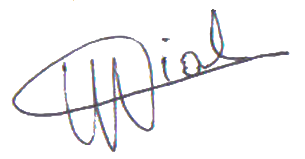
\includegraphics[width=3cm]{sig.png}
%

\newpage




\newgeometry{left=6.1cm,top=1.8cm,right=1.5cm,bottom=0.7cm,nohead,nofoot}



\header{Benjamin}{~Vial}{Posdoctoral Research Asssistant | Microwave Engineering and Photonics}

%----------------------------------------------------------------------------------------
%	SIDEBAR SECTION
%----------------------------------------------------------------------------------------

\begin{aside} % In the aside, each new line forces a line break
	\section{Contact}
	\faHome~~146 Glyn road
	London E5 0JE, UK
	\faPhone~~+44~7840~029~744
	\faEnvelope~~\href{mailto:b.vial@qmul.ac.uk}{b.vial@qmul.ac.uk}
	\faUser~~\href{http://bvial.info/}{bvial.info}
	\section{Information}
	date of birth 09/11/1984
	French citizenship
	\section{Languages}
	French mother tongue
	English fluent
	Spanish basic
	\section{Programming}
	\textbf{operating systems}
	Linux, Windows
	\textbf{languages and scripts}
	Python, Matlab, Mathematica, \LaTeX, C, C++, Q\#, HTML, CSS
	\textbf{applications}
	git, Comsol Multiphysics, Fenics, Gmsh, GetDP, Gimp, LibreOffice, Labview
	\section{Interests}
	\textbf{professional}
	Optics
	Photonics
	Metamaterials
	wave physics
	light-matter interraction
	homogenization methods
	computational EM
	numerical modelling
	optimization techniques
	inverse design
	finite element method
	Fourier modal method
	modal analysis
	machine learning
	Transformation Optics
	invisibility cloaking
	fabrication
	characterization
	open source science
	\textbf{personal}
	playing the guitar
	listening to music
	football, snowboard, hiking
	traveling, cooking
\end{aside}


%----------------------------------------------------------------------------------------
%	EDUCATION SECTION
%----------------------------------------------------------------------------------------

\section{Education}

\begin{entrylist}
	%------------------------------------------------
	\entry
	{Apr. 2013}
	{PhD {\normalfont in Physics}}
	{\href{http://www.fresnel.fr/}{Institut Fresnel}, CNRS, Centrale Marseille, Aix Marseille Universit\'e, Marseille, France}
	{Optics, Photonics and image processing}
	%------------------------------------------------
	\entry
	{Oct. 2009}
	{Master's degree {\normalfont in Physics}}
	{\href{http://www.centrale-marseille.fr/}{~~Centrale Marseille}~/~
		\href{http://www.lma.cnrs-mrs.fr/}{Laboratoire de Mécanique et d'Acoustique}, CNRS, Marseille, France}
	{Mechanics, Physics and Engineering, specialization in Acoustics}

	\entry
	{Oct. 2009}
	{Master's degree {\normalfont in Engineering}}
	{\href{http://www.centrale-marseille.fr/}{Centrale Marseille}, Marseille, France}
	{High level scientific and technical training}
	%------------------------------------------------
\end{entrylist}

%----------------------------------------------------------------------------------------
%	WORK EXPERIENCE SECTION
%----------------------------------------------------------------------------------------
\vspace*{-0.2cm}
\section{Research activities}

\begin{entrylist}
	%------------------------------------------------



	\entry
	{Jan. 2019 \\Now}
	{Postdoctoral Research Assistant}
	{\href{http://antennas.eecs.qmul.ac.uk/}{Queen Mary, University of London}, London, UK}
	{\href{https://animate-research.com/}{ANIMATE project}: nonlinear coupling model and homogenization of ferroelectric
		metamaterials, inverse design for tunability enhancement, microwave and THz material characterization.
	}


	\entry
	{Jan. 2017 \\Dec. 2018}
	{Postdoctoral Research Assistant}
	{\href{http://antennas.eecs.qmul.ac.uk/}{Queen Mary, University of London}, London, UK}
	{AOTOMAT project : Optimization tools and machine learning for the design of electromagnetic
		devices and materials.
	}

	\entry
	{Jul. 2014 \\Dec. 2016}
	{Postdoctoral Research Assistant}
	{\href{http://antennas.eecs.qmul.ac.uk/}{Queen Mary, University of London}, London, UK}
	{\href{http://www.quest-spatial-transformation.org/}{QUEST project: Quest for Ultimate Electromagnetics Using Spatial Transformations.}
		Transformation Optics applied to the design, fabrication and characterization of novel electromagnetic devices using metamaterials.
		Development of simulation tools and optimization techniques.
	}


	\entry
	{Nov. 2013\\ Jan. 2014}
	{Postdoctoral Research Assistant}
	{\href{http://www.fresnel.fr/}{Institut Fresnel}, Marseille, France}
	{
		Numerical study of the coupling of light
		to subwavelength resonant optical antennas and control of the local density of states.
	}
	%------------------------------------------------
	\entry
	{May 2013 \\Oct. 2013}
	{Postdoctoral Research Assistant}
	{\href{http://www.fresnel.fr/}{Institut Fresnel}, Marseille, France}
	{
		Development of simulation tools for ray tracing in complex media, inverse problem of
		finding index distribution to make light follow a prescribed path, deshomogenization
		technique with graded index photonic crystals.
	}

	%------------------------------------------------
	\entry
	{Oct. 2009\\Apr. 2013}
	{PhD in Physics}
	{\href{http://www.fresnel.fr/}{Institut Fresnel}~--~\href{http://www.silios.com/}{Silios Technologies}, Marseille, France}
	{\emph{\href{http://tel.archives-ouvertes.fr/index.php?halsid=slas337fv1oqlj1okgkq7q42i5&view_this_doc=tel-00918651&version=1}
			{Study of open electromagnetic resonators by modal approach.
				Application to infrared multispectral filtering.}} (\emph{joint academia/industry funding})\\
		FEM modelling of metamaterials, spectral analysis quasi-normal mode expansion.
		Application to the design of infrared filters for multispectral imaging devices.
		Fabrication and characterization of reflexion bandcut and transmission bandpass filters.
	}

\end{entrylist}

%----------------------------------------------------------------------------------------
%	Teaching/supervising experience SECTION
%----------------------------------------------------------------------------------------

\vspace*{-0.2cm}
\section{Teaching/supervising experience}

\begin{entrylist}
	%------------------------------------------------
	\entry
	{2011-2012}
	{Internship supervisor}
	{{Institut Fresnel}, CNRS, Centrale Marseille, Marseille, France}
	{Optimization of diffractive spectral infrared filters (1 engineer student, 6 months).\\
		Optimization of absorption in solar cells (4 engineer students, 3 months).
	}

	%------------------------------------------------
	\entry
	{2019}
	{Teaching Assistant}
	{\href{http://antennas.eecs.qmul.ac.uk/}{Queen Mary, University of London}, London, UK}
	{Quantum Programming. Lectures and tutorials on quantum gates and circuits.
		Coding laboratory and projects in Q\# an Python (10 Master students, 6 months).}

	%------------------------------------------------

\end{entrylist}

\vspace*{-0.2cm}
\section{Awards and honours}

  {Best PhD thesis 2014 award} from the {\href{https://ecole-doctorale-352.univ-amu.fr/en}{Doctoral School 352, Physics and Condensed Matter Science}}

  {Best PhD thesis 2014 award from {\href{https://www.cnano-paca.fr/index.php?option=com_content&view=article&id=80}{CNano PACA}}, finalized research category}



\newgeometry{left=1.5cm,top=1.8cm,right=1.5cm,bottom=0.7cm,nohead,nofoot}



%----------------------------------------------------------------------------------------
%	Referees contact SECTION
%----------------------------------------------------------------------------------------


\section{References}

Available on request.
% 
% \section{Referees contact}
% 
% \begin{minipage}{.6\textwidth}
% 	\textbf{Prof Yang Hao}\\
% 	\faHome~~School of Electronic Engineering and Computer Science\\
% 	Queen Mary University of London\\
% 	Peter Landin Building, 10 Godward Square, Mile End Road\\
% 	London E1 4FZ, United Kingdom\\
% 	\faEnvelope~~\href{mailto:y.hao@qmul.ac.uk}{y.hao@qmul.ac.uk}\\
% 	\faPhone~~+44 20 7882 5341\\
% 	\faUser~~\href{http://www.eecs.qmul.ac.uk/~yang/}{www.eecs.qmul.ac.uk/~yang/}
% \end{minipage}%
% \begin{minipage}{0.4\textwidth}
% 	\textbf{Prof Andr\'e Nicolet}\\
% 	\faHome~~Aix-Marseille Université\\
% 	Institut Fresnel (UMR CNRS 6133)\\
% 	Domaine Universitaire de Saint-Jérôme\\
% 	F13397 Marseille cedex 20, France\\
% 	\faEnvelope~~\href{mailto:andre.nicolet@fresnel.fr}{andre.nicolet@fresnel.fr}\\
% 	\faPhone~~+33 4 91 28 87 73\\
% 	\faUser~~\href{https://www.fresnel.fr/perso/nicolet/}{www.fresnel.fr/perso/nicolet/}
% \end{minipage}


\vspace*{0.5cm}

%----------------------------------------------------------------------------------------
%	Publications SECTION
%----------------------------------------------------------------------------------------


\section{Publications}

\printbibsection{article}{Articles in peer-reviewed journals}

\printbibsection{book}{Contribution to book chapter}

\printbibsectionkey{inproceedings}{Proceedings of international peer-reviewed conferences}{lecture comittee}

\printbibsectionkey{inproceedings}{International peer-reviewed conferences}{conference}

\printbibsectionkey{misc}{PhD thesis}{phdthesis}

\printbibsectionkey{misc}{Open source software and code}{code}

\printbibsectionkey{misc}{In preparation}{prep}


\end{document}
